\chapter{Результаты}
Примеры работы программы приведены на рисунках \ref{p1}--\ref{p4}.

\begin{figure}[h]
	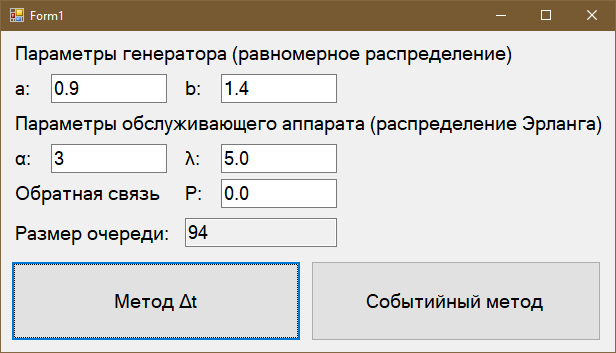
\includegraphics[width=1\linewidth]{inc/img/1.png}
	\caption{Принцип $\Delta$t без обратной связи}
	\label{p1}
\end{figure}

\newpage
\begin{figure}[h]
	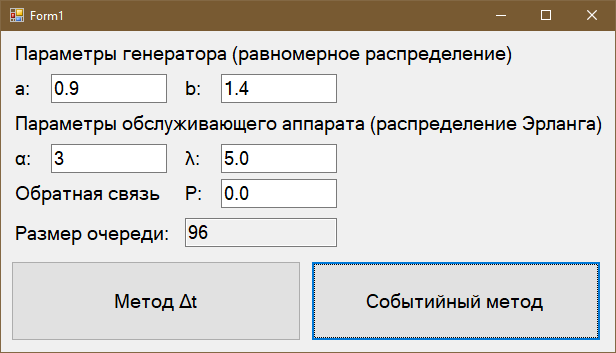
\includegraphics[width=1\linewidth]{inc/img/2.png}
	\caption{Событийный принцип без обратной связи}
	\label{p2}
\end{figure}

По рисункам \ref{p1} и \ref{p2} видно, что результаты обоих принципов примерно одинаковы.

\newpage
\begin{figure}[h]
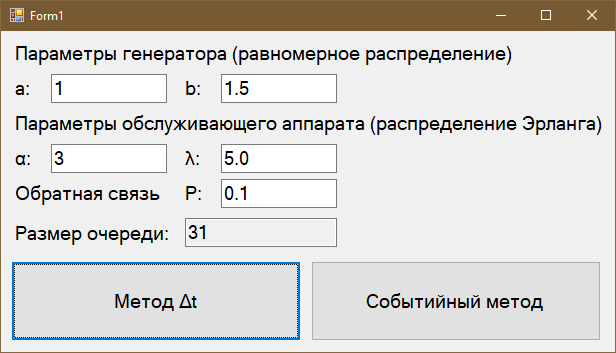
\includegraphics[width=1\linewidth]{inc/img/3.png}
\caption {Принцип $\Delta$t c обратной связью}
\label{p3}
\end{figure}

\begin{figure}[!h]
	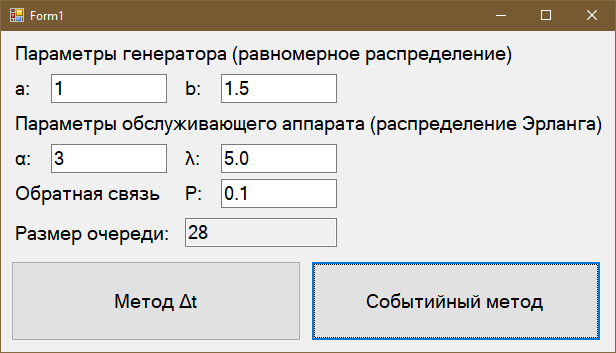
\includegraphics[width=1\linewidth]{inc/img/4.png}
	\caption{Событийный принцип c обратной связью = 1}
	\label{p4}
\end{figure}

Как видно на рисунках \ref{p3} и \ref{p4} при обратной связи результаты разных методов также похожи.

\newpage
\begin{figure}[h]
	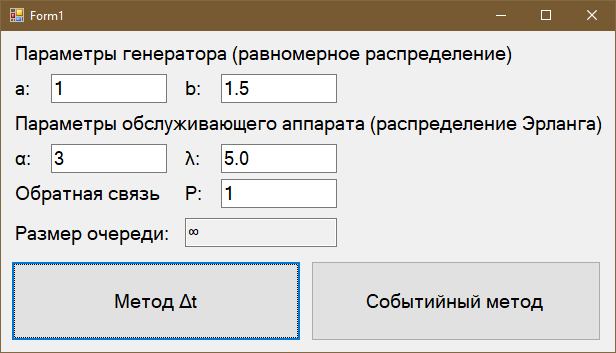
\includegraphics[width=1\linewidth]{inc/img/5.png}
	\caption {Принцип $\Delta$t c обратной связью}
	\label{p5}
\end{figure}

\begin{figure}[!h]
	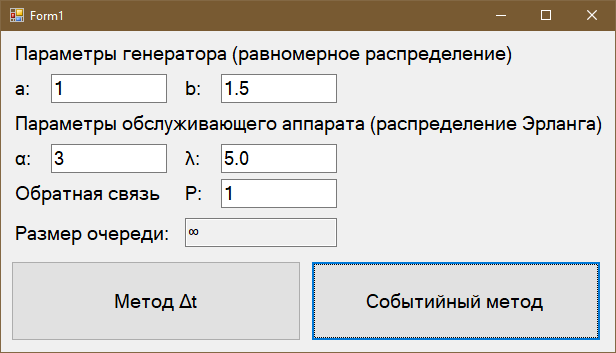
\includegraphics[width=1\linewidth]{inc/img/6.png}
	\caption{Событийный принцип c обратной связью = 1}
	\label{p6}
\end{figure}

Очевидно что при обратной связи равной 1, потери сообщений не избежать вне зависимости от используемого метода, что видно на рисунках \ref{p5} и \ref{p6}.